  \let\negmedspace\undefined
\let\negthickspace\undefined
\documentclass[journal]{IEEEtran}
\usepackage[a5paper, margin=10mm, onecolumn]{geometry}
%\usepackage{lmodern} % Ensure lmodern is loaded for pdflatex
\usepackage{tfrupee} % Include tfrupee package

\setlength{\headheight}{1cm} % Set the height of the header box
\setlength{\headsep}{0mm}     % Set the distance between the header box and the top of the text

\usepackage{gvv-book}
\usepackage{gvv}
\usepackage{cite}
\usepackage{amsmath,amssymb,amsfonts,amsthm}
\usepackage{algorithmic}
\usepackage{graphicx}
\usepackage{textcomp}
\usepackage{xcolor}
\usepackage{txfonts}
\usepackage{listings}
\usepackage{enumitem}
\usepackage{mathtools}
\usepackage{gensymb}
\usepackage{comment}
\usepackage[breaklinks=true]{hyperref}
\usepackage{tkz-euclide} 
\usepackage{listings}
% \usepackage{gvv}                                        
\def\inputGnumericTable{}                                 
\usepackage[latin1]{inputenc}                                
\usepackage{color}                                            
\usepackage{array}                                            
\usepackage{longtable}                                       
\usepackage{calc}                                             
\usepackage{multirow}                                         
\usepackage{hhline}                                           
\usepackage{ifthen}                                           
\usepackage{lscape}
\begin{document}

\bibliographystyle{IEEEtran}
\vspace{3cm}

\title{9.7.11}
\author{EE24BTECH11058 - P.Shiny Diavajna}
% \maketitle
% \newpage
% \bigskip
{\let\newpage\relax\maketitle}

\renewcommand{\thefigure}{\theenumi}
\renewcommand{\thetable}{\theenumi}
\setlength{\intextsep}{10pt} % Space between text and floats


\numberwithin{equation}{enumi}
\numberwithin{figure}{enumi}
\renewcommand{\thetable}{\theenumi}


\textbf{Question}: Find a particular solution of the differential equation, given that
$y=-1$ when $x=0$.
\begin{align}
  \brak{x-y}\brak{dx+dy}=dx-dy
\end{align}

\textbf{Theoretical solution:}
 \begin{align}
 (x-y-1)dx&=(-x+y-1)dy\\
 \frac{dy}{dx}&=-\brak{\frac{x-y-1}{x-y+1}}\\
 \text{Let } x-y&=t\\
 1-\frac{dy}{dx}&=\frac{dt}{dx}
\end{align}

Substitute equations (0.4) and (0.5) in (0.3)

\begin{align}
    1-\frac{dt}{dx}&=-\brak{\frac{t-1}{t+1}}\\
    \frac{dt}{dx}&=\frac{2t}{t+1}\\
    \frac{t+1}{2t} dt&=dx
\end{align}

Integrating on both sides 
\begin{align}
\int \brak{\frac{1}{2} + \frac{1}{2t}} \, dt &= \int dx\\
\frac{t}{2}+\frac{1}{2}\ln{|t|} &=x+c
\end{align}

Substitute $t=x-y$

\begin{align}
      \frac{x-y}{2}+\frac{1}{2}\ln{|x-y|}&=x+c
\end{align}

Given, x=0,y=-1.On substitution in (0.11) ,c=$\frac{1}{2}$
\begin{align}
    \ln{|x-y|}=x+y+1
\end{align}

\textbf{Method of finite differences :}
The finite difference method is rooted in the fundamental concept of approximating derivatives using finite differences.

The derivative of $y(x)$ can be approximated as 
\begin{align}
    \frac{dy}{dx}&=\frac{y(x+h)-y(x)}{h}\\
    y(x+h)&=y(x)+h\brak{\frac{dy}{dx}}
\end{align}
Where h is a small value very close to zero.

Substitute (0.3) in (0.14)
\begin{align}
    y(x+h)=y(x)-h \brak{\frac{x-y-1}{x-y+1}}
\end{align}

Let \brak{x_0,y_0} be a point on the curve.\\
Let some $x_1=x_0 +h$.Then,
\begin{align}
    y_1 = y_0-h \brak{\frac{x-y-1}{x-y+1}}
\end{align}

On Generalizing the above equation, we have 
\begin{align}
    x_{n+1}&=x_{n} +h \\
    y_{n+1}&=y_{n}-h \brak{\frac{{x_n}-{y_n}-1}{{x_n}-{y_n}+1}} 
\end{align}

This curve is generated by applying the finite difference method to the given problem and taking the values of $x_0=0,y_0=-1$ and $h=0.001$ and running the iterations for 500 times 
\begin{figure}[h]
   \centering
   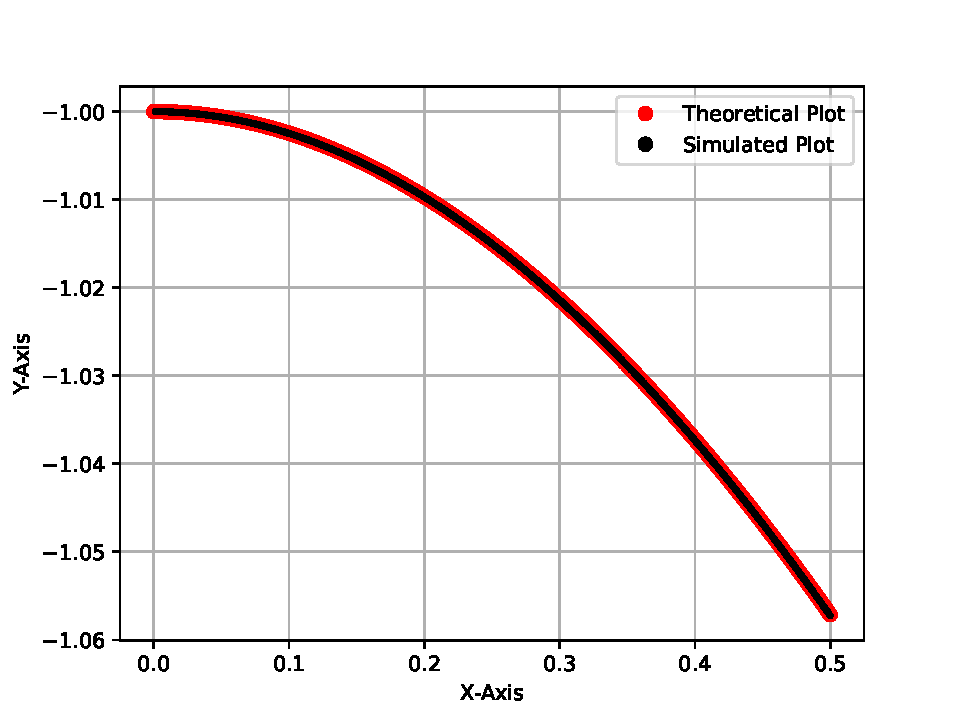
\includegraphics[width=\columnwidth]{figs/fig.pdf}
\end{figure}


\end{document}
